\chapter{Theoretical overview}
\label{chap:Theory}

\chapterquote{ILC will be built next year}%
{Mysterious person}%: Blackwood's Magazine May 1830

This chapter provides a theoretical overview which would be used in the subsequent  chapters. A short review of the Standard Model of Particle Physics, the current best particle theory, is provided, with an emphasis on the Higgs mechanism and the Higgs boson. A general parametrisation of the Higgs theory, beyond the Standard Model, is discussed, and supplies the theoretical background for the physics analysis in the \Chapter{chap:DoubleHiggs}.

\section{Overview of the Standard Model}

The Standard Model (\SM) is a quantum field theory concerning three fundamental interactions of nature: the electromagnetic, weak and strong integrations. The \SM also describes the interactions between the sub-atomic particles. The deployment and the experimental verification of the \SM throughout the second half of the 20th century is one of the greatest triumph of the particle physics. The most recent discovery of the Higgs boson in 2012 \cite{Aad:2012tfa} further verified the theory. This chapter summarise the \SM based on the summaries of the \SM \cite{Agashe:2014kda,Thomson:2013zua,Tong:QFT,Gripaios:GFT}.

The fundamental particles in the \SM consist of three categories: force exchange bosons, leptons and neutrinos, and quarks. In the \SM, the force exchange bosons carries the fundamental forces between particles. For example, photon is the force carrier of the electromagnetic force. \PWp, \PWm, and \PZ are the force carriers of the weak force. Gluon, \Pg, is the force carrier of the strong force. These bosons will be discussed further in \Section{sec:theoryElectroweak}. There is also the Higgs boson from the spontaneous symmetry breaking of the Higgs filed, which is discussed in \Section{sec:theoryHiggsBoson}

%A summary of the selected properties of these force exchange bosons can be found in \Table{}.

Another category of fundamental particles contains leptons and neutrinos. These particles are fermions. For each fermion in the \SM, there is an anti-fermion with same mass and spin, but opposite charge. Leptons and neutrinos have three generations. Each generation has same interaction properties, but different masses. Although neutrinos could not be directly detected, measurements of the \PZ decay width strong suggested the three generations of neutrinos \cite{ALEPH:2005ab}. Leptons and neutrinos experience weak forces as well as electromagnetic forces, which will be further discussed in \Section{sec:theoryElectroweak}.

The last category of fundamental particles are quarks, which are also fermions and have three generations. Each generation has a positively charged up type quark and a negatively charged down type quark. Quarks experiences all three fundamental forces described by the \SM.

The \SM has enjoyed great success with theoretical predictions being experimentally varied. Some highlights included the discovery of the top quark in 1995 cite{}, the tau netrino in 2000 cite{} and the Higgs bosons in 2012 cite{Aad:2012tfa}. However, there are observations which are not explained by the \SM. One issue is that the \SM does not incorporate the gravitational force. There have been attempts to modify the \SM but no conclusive theory yet. Another issue is that the \SM does not allow neutrino masses and mixings. There have been many theories beyond the Standard Model (BSM). One such example is the generalisation of the Higgs theory to allow non \SM coupling strengths. This will be discussed in \Section{sec:theoryHiggsBSM}.

Notations and conventions will be introduced. The overview of the Standard Model starts with the quantum electrodynamics, and its generalisation to quantum chromodynamics. The unification of electromagnetism and weak interaction, electroweak gauge theory will be discussed. Afterwards, Higgs mechanism and Yukawa couplings will be introduced to explain bosons and fermions masses whilst preserving the Lagrangian symmetry. This will be followed by a detailed discussion on the Standard Model Higgs boson, its mass and interactions with other particles. The chapter finishes with explanation for possible Higgs theories beyond the Standard Model, the Lagrangian of the Higgs interaction, and observables, which forms the theoretical background for the analysis on the double Higgs production in the \Chapter{chap:DoubleHiggs}.


\section{Notations and conventions}

The natural unit is used in this document, $\hbar = c = 1$. The metric is mostly-minus, $\eta^{\mu\nu} = \text{diag}(1,-1,-1,-1)$. The Dirac gamma matrices are represented with $\gamma^{\mu}$, with $\mu$ goes from 0 to 3. $\gamma^5 = i \gamma^{0}\gamma^{1}\gamma^{2}\gamma^{3}$. $\overline{\psi} = \psi^{\dagger}\gamma^0$. Einstein summation convention is used as well this document.

This set of notations allows a contracted pair to be a Lorentz invariant. For a Weyl spinor, $\psi_\alpha$, the mass term in the lagrangian is of the form $\psi^{\alpha}\psi_\alpha$, which is the Majorana mass term. The contracted pair between two different Weyl spinors would form a Dirac mass term.


\section{Quantum electrodynamics}

The natural starting point to introduce the \SM is the quantum electrodynamics (\QED). The \QED is a quantum field theory explaining electromagnetic interactions. The theory involves a spin-half Dirac (electron) field $\psi$ and a vector (photon) field $A_{\mu}$. When the local (gauge) symmetry is imposed, which is equivalent to the Lagrangian invariance under transformations,
\begin{equation}
\psi\ \to\ e^{ie\phi(x)},\ A_{\mu}\ \to\ A_{\mu} - \partial^{\mu}\phi(x),
\end{equation}
the Lagrangian is fixed to be
\begin{equation}
\Lagr_{QED} = \overline{\psi} \left( i\Dstroke - m \right)\psi -  \frac{1}{4}F_{\mu\nu}F^{\mu\nu},
\end{equation}
if up to cubic terms are allowed in the fields. There are two free parameters in the \QED, $m$ the electron mass, and $e$ the electron charge. The mass term for the photon, $\nu^{2}A_{nu}A^{\nu}$, is forbidden by gauge invariance.

The \QED has been verified experimentally. One of the greatest prediction is the spin magnetic dipole moment of the electron, defined as $\vec{\mu} = g_{s}\frac{Qq}{2m} \vec{s}$. The $g_{s}$ is predicted to be 2 by the Dirac equations. The small corrections to the value comes from the electron's interaction with virtual photons, so called higher ``loop'' corrections in Feynman diagrams. The precise agreement of the theoretical prediction and the experimental value is a success of the \QED.

\begin{comment}
The Standard Model of particle physics is a theory concerning the electromagnetic, weak, and strong interactions, as well as classifying all the elementary particles known. It was developed throughout the latter half of the 20th century, as a collaborative effort of scientists around the world.[1] The current formulation was finalized in the mid-1970s upon experimental confirmation of the existence of quarks. Since then, discoveries of the top quark (1995), the tau neutrino (2000), and the Higgs boson (2012) have given further credence to the Standard Model. Because of its success in explaining a wide variety of experimental results, the Standard Model is sometimes regarded as the "theory of almost everything".

Although the Standard Model is believed to be theoretically self-consistent[2] and has demonstrated huge and continued successes in providing experimental predictions, it does leave some phenomena unexplained and it falls short of being a complete theory of fundamental interactions. It does not incorporate the full theory of gravitation[3] as described by general relativity, or account for the accelerating expansion of the Universe (as possibly described by dark energy). The model does not contain any viable dark matter particle that possesses all of the required properties deduced from observational cosmology. It also does not incorporate neutrino oscillations (and their non-zero masses).

The development of the Standard Model was driven by theoretical and experimental particle physicists alike. For theorists, the Standard Model is a paradigm of a quantum field theory, which exhibits a wide range of physics including spontaneous symmetry breaking, anomalies and non-perturbative behavior. It is used as a basis for building more exotic models that incorporate hypothetical particles, extra dimensions, and elaborate symmetries (such as supersymmetry) in an attempt to explain experimental results at variance with the Standard Model, such as the existence of dark matter and neutrino oscillations.
\end{comment}

\section{Quantum chromodynamics}

Like the \QED, the quantum chromodynamics (\QCD) a quantum field theory explaining strong interactions. There are eight gauge bosons, gluons, coupling to nine fermions, quarks. Unlike the \QED, the theory is invariant under local non-Abelian SU(3) transformations. Gulons can interact with other gluons, and carry colour charge (red, green, and blue). Nine quarks transform as colour triplets. The \QCD Lagrangian is
\begin{equation}
\Lagr_{QCD} = \sum_{f\in{u,d,s,c,b,t}} \overline{\psi} \left( i\gamma^{\mu}\partial_{\mu} - g_{s}\gamma^{\mu}G^a_{\mu}\frac{\lambda^a}{2} - m_f \right)\psi -  \frac{1}{4}G^a_{\mu\nu}G^{a\mu\nu},
\end{equation}
where $g_s$ is the strong coupling constant. $a$ is the colour charge. $\lambda$ is the Gell-Mann matrices. $G^a_{\mu\nu}$ is the gluon field strength, given by
\begin{equation}
G^a_{\mu\nu} = \partial_{\mu}\gamma_{\nu}^a - \partial_{\nu}\gamma_{\mu}^a  - g_{s}f_{abc}G_{\mu}^{b}G_{\nu}^c.
\end{equation}
The last extra term comparing to \QED indicates the non-Abelian nature of the \QCD.

\section{The electroweak interaction}
\label{sec:theoryElectroweak}
The electroweak interaction can be thought of a extension to the \QED to incorporate the weak force, and to explain different coupling strength to left-handed and right-handed fermions. However, the Lagrangian  does not allow the massive  electroweak force exchange bosons and fermions, which are explained by the Higgs mechanism  and  the Yukawa interactions.

There are four vector boson fields in the theory, 3 $W$ and 1 $B$ field. The Lagrangian can be divided into two parts: the bosonic self interaction and the couplings to the fermions.
\begin{equation}
\Lagr_{Electroweak} = \Lagr_{Boson} + \Lagr_{Fermion}
\end{equation}

The bosonic self interaction Lagrangian, $\Lagr_{Boson}$, is given by
\begin{equation}
\Lagr_{Boson} = - \frac{1}{4} W^i_{\mu\nu} W^{i\mu\nu} - \frac{1}{4}B_{\mu\nu} B^{\mu\nu},
\end{equation}
where
\begin{equation}
W^i_{\mu\nu} = \partial_{\nu}W^i_{\mu} - \partial_{\mu}W^i_{\nu} - g\varepsilon^{ijk}W^j_{\mu}W^k_\nu
\end{equation}
\begin{equation}
B_{\mu\nu} = \partial_{\nu}B_{\mu} - \partial_{\mu}B_{\nu}
\end{equation}
$B$ field  is invariant under U(1). $W$ field is invariant under non-Abelian SU(2) transformations. $g$ is the coupling strength of the $W$ field. The indices, i, j, and k indicates 3 $W$ fields, going from 1 to 3.

The fermionic part of the Lagrangian,   $\Lagr_{Fermion}$, has different components for the left-handed and right-handed fermions, given by
\begin{equation}
\Lagr_{Fermion} = \sum_{\psi\in{fermions}} {\overline{\psi}}_L \gamma^{\mu}D^L_{\mu} \psi_L +  \overline{\psi}_R \gamma^{\mu}D^R_{\mu} \psi_R
\end{equation}
$D^L_{\mu}$ and $D^R_{\mu}$ are defined as
\begin{equation}
D^L_{\mu} = \partial_{\mu} + ig\frac{\tau_i}{2}W^i_{\mu} + ig'Y_{\psi}B_{\mu}
\end{equation}
\begin{equation}
D^R_{\mu} = \partial_{\mu}  + ig'Y_{\psi}B_{\mu}
\end{equation}
This Lagrangian allows $W$ and $B$ field to couple with left-handed fermions, but only $B$ field couples to right-handed fermions. The $\tau_i$ matrices are the generators of the SU(2). Pauli spin matrices are one of the representations. $Y_{\psi}$ is the hypercharge associating with the fermion field $\psi$. $g'$ is the $B$ field strength.

Physical bosons \PWp, \PWm  only couples to left-handed fermions. \PZ and \Pgamma couples to both left-handed and right-handed fermions. Hence $W^1$ and $W^2$ are associated to \PWp and \PWm. Mass eigenstates for \PZ and \Pgamma, $Z_{\mu}$ and $A_{\mu}$ are mixture of $W^3_{\mu}$ and $B_{\mu}$.
\begin{equation}
Z_{\mu} = \cos\left(\theta_W\right)W^3_{\mu} - \sin\left(\theta_W\right)B_{\mu}
\end{equation}
\begin{equation}
A_{\mu} = \sin\left(\theta_W\right)W^3_{\mu} + \cos\left(\theta_W\right)B_{\mu}
\end{equation}
$\theta_W$ is the Weinberg mixing angle \cite{Weinberg:1967tq}, which is determined experimentally. So far the SU(2)$\otimes$U(1) gauge theory explains the parity violating nature of the weak interaction. The explicit fermion mass are not allowed in the gauge symmetry. The higgs mechanism via spontaneous symmertry breaking would introduce mass terms for fermions.

\section{Higgs Mechanism}
\label{sec:theoryHiggs}
A complex  scalar Higgs field, $\Phi_H$, is added to the electroweak Lagrangian. $\Phi_H$ transforms as a doublet of SU(2) with hypercharge $Y = \frac{1}{2}$
\begin{equation}
\Lagr_{Higgs} = \left(D_\mu\Phi_H\right)^\dagger\left(D^\mu\Phi_H\right) - \mu^2\Phi_H^\dagger\Phi_H - \lambda\left(\Phi_H^\dagger\Phi_H\right)^2
\end{equation}
with
\begin{equation}
D_\mu\Phi_H = \left(\partial_{\mu} + ig\frac{\tau_i}{2}W^i_{\mu} + ig'\frac{1}{2}B_{\mu}\right)\Phi_H
\end{equation}
For negative $\mu^2$, the Higgs filed potential
\begin{equation}
\mu^2\Phi_H^\dagger\Phi_H + \lambda\left(\Phi_H^\dagger\Phi_H\right)^2
\end{equation}
is minimised with a Higgs vacuum potential $\frac{\nu}{\sqrt{2}}=\sqrt{\frac{\nu^2}{2\lambda}} $. After the symmetry breaking, the $\Lagr_{Higgs}$ provides  the mass terms for \PWp, \PWm, \PZ and \Pgamma via terms in the Lagrangian:
\begin{equation}
\frac{{\left(g\nu\right)}^2}{4}W^+_{\mu}W^{-\mu} + \frac{\left(g^2 + g^{'2}\right)\mu^2}{8}Z_{\mu}Z^{\mu}
\label{eq:theoryBoson}
\end{equation}
This provides equal mass for \PWp and \PWm with massless photon.

\section{Yukawa couplings}

\SECTION{sec:theoryHiggs} explains the Higgs mechanism for gauge bosons gaining masses. The fermions gain masses in a similar fashion. Consider a Higgs field transforming as a doublet of SU(2) with hypercharge $Y = \frac{1}{2}$, the Yukawa couplings is given

\begin{equation}
\Lagr_{Yukawa} = -\lambda^{u}\overline{q_L}\Phi_H^{c}u_R - -\lambda^{d}\overline{q_L}\Phi_H{d}_R - \lambda^{e}\overline{l_L}\Phi_{H}e_R + h.c.
\end{equation}
$\Phi_H^{c} \equiv i \sigma^2H^*$ is an SU(2) double field with hypercharge $Y = -\frac{1}{2}$ and $\sigma$ is the Pauli spin matrix. $u$, $d$, and $e$ are fields for up-type quark, down-type quark and leptons. The Lagrangian is summed over all possible quarks and leptons. The interactions terms in the $\Lagr_{Yukawa}$ become mass terms when the Higgs vacuum expectation value is substituted. The fermion masses are given by
\begin{equation}
m_{u} = \frac{\lambda^u{\nu}}{\sqrt{2}},\ m_{d} = \frac{\lambda^d{\nu}}{\sqrt{2}},\ m_{e} = \frac{\lambda^e{\nu}}{\sqrt{2}}
\end{equation}

\section{Standard Model Higgs boson}
\label{sec:theoryHiggsBoson}
So far, interactions between different fields in the Standard Model, as well as the mass obtaining mechanism have been discussed. Only left for discussion is the Higgs bosons, and its interactions with other fields.

For the Higgs doublet complex field in the \SM, there are four real scalar degrees of freedom. By choosing the unitary gauge, three degree of freedoms are manifestly eaten. The Higgs field becomes
\begin{equation}
H(x) = \frac{1}{\sqrt{2}}
 \begin{pmatrix}
  0 \\
  \nu + h(x) \\
 \end{pmatrix}
\end{equation}
$h(x)$ is real scalar field for the Higgs boson. It is not charged under electromagnetism as it is real. The Higgs boson interaction terms in the Lagrangian  with other particles can be shown by replacing $\nu$  with $\nu + h(x)$ in previous expressions. For fermions  field, $\psi_i$, the Higgs boson interaction term is given by
\begin{equation}
\Lagr\supset-\frac{m_i}{\nu}h\overline{\psi}_i\psi_i
\end{equation}

From the \Equation{eq:theoryBoson}, the Higgs boson interaction terms for bosons can be shown as
\begin{equation}
\label{eq:theoryHiggsBosonic}
\Lagr\supset m^2_W\left(\frac{2h}{\nu} + \frac{{h}^2}{\nu^2}\right)W^+_{\mu}W^{-\mu} + \frac{m^2_Z}{2}\left(\frac{2h}{\nu} + \frac{{h}^2}{\nu^2}  \right)Z_{\mu}Z^{\mu}
\end{equation}
The Higgs boson self interactions are obtained from the Higgs field potential
\begin{equation}
\label{eq:theoryHiggsSelfCoupling}
\Lagr\supset \frac{\mu^2}{2}\left(\nu+h\right)^2 - \frac{\lambda}{4}\left(\nu+h\right)^4 \supset -\lambda\nu^2{h}^2-\lambda\nu{h}^3 - \frac{\lambda}{4}h^4 = -\frac{m_h^2}{2}h^2 - \frac{m_h^2}{2\nu}h^3 - \frac{m_h^2}{8\nu^2}h^4.
\end{equation}
The Higgs boson mass, $m_h$ is $2\lambda\nu^2$. The triple and quartic self interaction strengths are $- \frac{m_h^2}{2\nu}$ and $\frac{m_h^2}{8\nu^2}$. Once the $m_h$ is determined, $\lambda$ can be worked out. The Higgs boson decay width and branching fraction can be roughly worked out. For example, \Figure{fig:theoryHiggsDecayWidth} and \Figure{fig:theoryHiggsBranchingRatio} show partial decay width and the branching ratios as a function of $m_h$.

The Higgs boson decaying to a pair of heavier particles, such as $\PWp\PWm$ or \PZ\PZ is forbidden kinematically. However, \Figure{fig:theoryHiggsPhenomenology} shows that the Higgs decaying to  $\PWp\PWm$  dominates before the mass threshold $m_H = 2m_W \sim 160 \ GeV$. This is because one of the $\PWpm$ gauge bosons is virtual and not on the mass shell, which is allowed by the quantum field theory. The virtual gauge boson subsequently decays to real on-shell particles.

%Higgs prefers to decay to the most massive possible final state. The ratio of fermionic branching ratios are proportional to fermion masses squared, modulo color factors and radiative corrections.
\begin{figure}[tbph]
\centering
    \begin{subfigure}[b]{0.45\textwidth}
        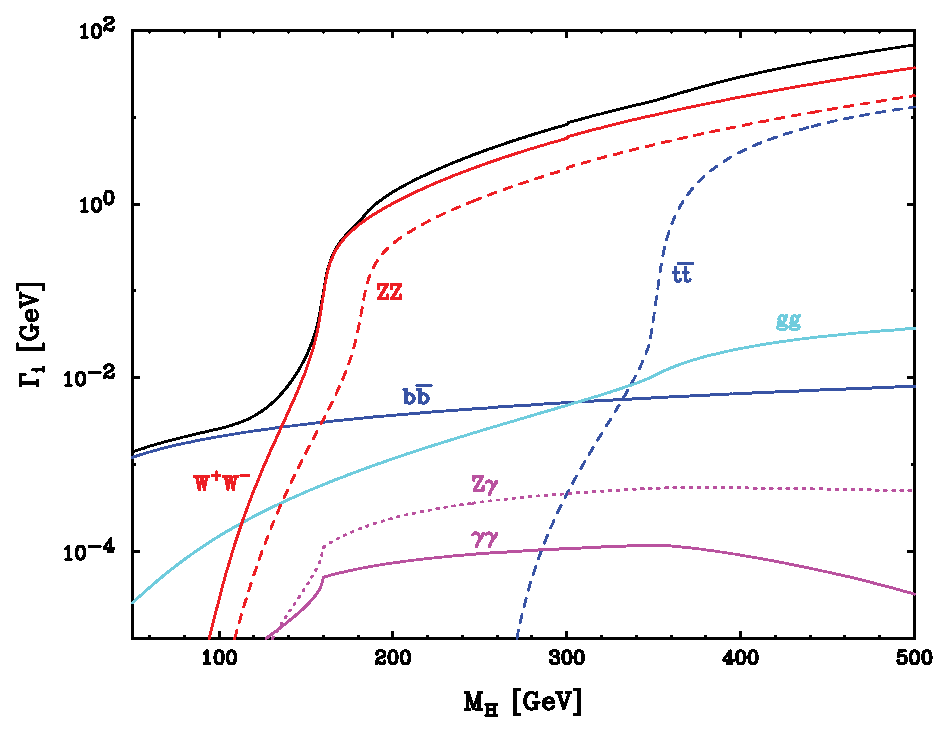
\includegraphics[width=\textwidth]{theory/HiggsDecayWidth}
        \caption{}
        \label{fig:theoryHiggsDecayWidth}
    \end{subfigure}
    \begin{subfigure}[b]{0.45\textwidth}
        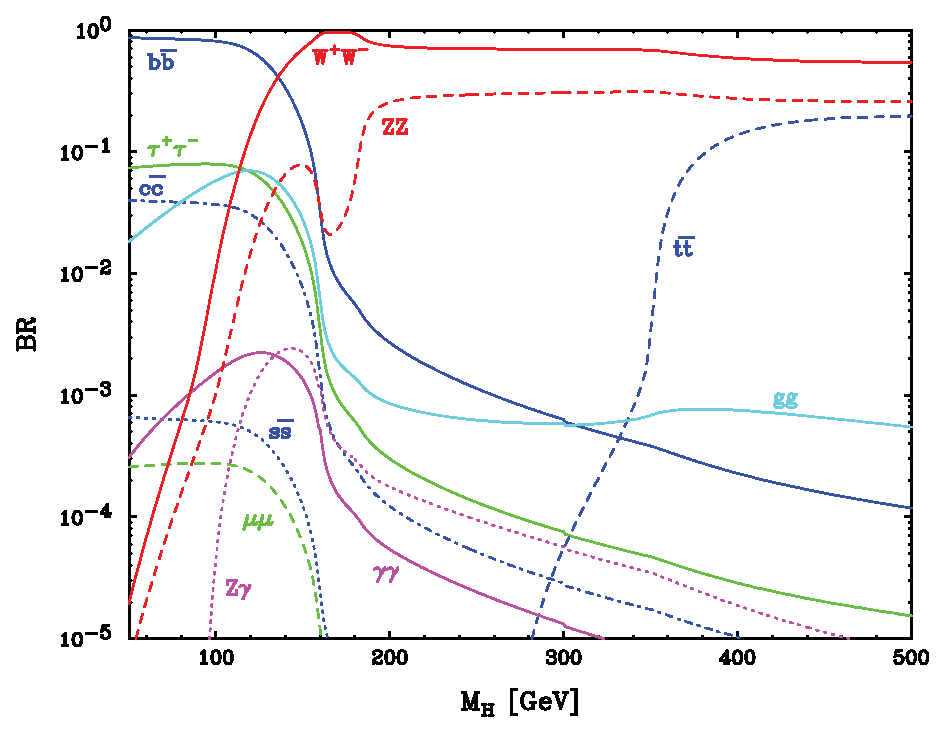
\includegraphics[width=\textwidth]{theory/HiggsBranchingRatio}
        \caption{}
        \label{fig:theoryHiggsBranchingRatio}
    \end{subfigure}
\caption[]
{\Figure{fig:theoryHiggsDecayWidth} shows Standard Model Higgs boson partial widths as a function of its mass, $M_H$. The total width is the black curve \Figure{fig:theoryHiggsBranchingRatio} shows selected Standard Model Higgs boson branching ratios as a function of its mass, $M_H$. Both plots are taken from \cite{Rainwater:2007cp} }
\label{fig:theoryHiggsPhenomenology}
\end{figure}


\section{Higgs beyond the Standard Model}
\label{sec:theoryHiggsBSM}

Since the \SM like Higgs boson discovery in 2012, it becomes important to understand of role of the Higgs boson in the electroweak spontaneous symmetry breaking. In the absence of the Higgs boson, the coupling strength of the longitudinally polarised vector bosons grows with energy and becomes strong at TeV scale. The \SM Higgs bosons moderates the interacting strength, allowing the extraction of the weak coupling at short distances. In this scenario, the \SM Higgs couplings are constrained and predicted in one parameter only, the Higgs mass. But other alternative scenarios could allow the behaviour of the \SM Higgs at low energy. One such example, motivated by the hierarchy problem and the electroweak data, is that the light and narrow Higgs-scalar is a composite bound state of some strongly interacting sector at the TeV scale. The couplings of the Higgs to fermions and bosons would be different to those in the \SM. If the composite Higgs is the pseudo Nambu-Goldstone boson from a spontaneous global symmetry breaking, the Higgs can be naturally light \cite{Kaplan:1983fs}. Another scenario is that a composite dilaton, the pseudo Nambu-Goldstone boson arose from a spontaneous scale invariance breaking, partially behaves like a light Higgs \cite{Goldberger:2008zz}. In both scenarios, the interaction of Higgs becomes strong at high energy. The coupling of the Higgs would deviate to those in the \SM.

An important physics channel for testing the Higgs theory is the double Higgs production via vector boson fusion at high energy \cite{Giudice:2007fh,Contino:2010mh,Contino:2013gna}. For the composite Higgs scenario, the scattering amplitude increases with the energy. For the dilaton scenario, no energy defence on the scattering amplitude is expected. It is difficult for the Large Hardon Collider to measure the cross section due to the large \SM background rate \cite{Contino:2010mh}. However, a multi-TeV linear electron position collider, such as Compact Linear Collider, would be able to precisely measure the cross section \cite{Barger:2003rs}.

Following the assumption made in the \cite{Contino:2010mh,Contino:2013gna}, the self interaction of the light scalar Higgs, $h$, and its coupling to other \SM bosons can be described by the following Lagrangian. The notation in the \cite{Contino:2013gna} is followed. After the electroweak symmetry breaking, the bosonic part of the Lagrangian reads:
\begin{equation}
\Lagr =\frac{1}{2}\left(\partial_\mu{h}\right)  - V(h) + \parenths{m_W^2{W}_\mu^+{W}^{-\mu} + \frac{m_Z^2}{2}Z_{\mu}Z^\mu}\sqbracs{1 + 2a\frac{h}{\nu} + b \frac{h^2}{\nu^2} + \hdots},
\end{equation}
where $V(h)$ is the $h$ field potential,
\begin{equation}
V(h) = \frac{1}{2}m_h^2h^2 + d_3\parenths{\frac{m_h^2}{2\nu}}h^3 + d_4\parenths{\frac{m_h^2}{8{\nu}^2}}h^4 + \hdots .
\end{equation}
$a$, $b$, $d_3$ and $d_4$ are arbitrary dimensionless parameters. Higher order terms in $h$ are omitted. $a$ and $b$ are proportional to the coupling strength of the $VVh$ and $VVhh$ vertices, where $V = \PWpm, \PZ$. $d_3$ and $d_4$ are proportional to the triple and quartic $h$ self coupling strength. Comparing with \Equation{eq:theoryHiggsBosonic} and \Equation{eq:theoryHiggsSelfCoupling}, the \SM Higgs suggests $a=b=d_3=d_4=1$ and all higher order terms vanish. The dilaton scenario imposes the relation, $a = b^2$.

The scattering amplitude for \HepProcess{{V}_L{V}_L \to hh} can be written as
\begin{equation}
A = a^2\parenths{A_{SM} + A_1\delta_b + A_2\delta_{d_3}},
\end{equation}
where $A_{SM}$ is the \SM amplitude and 
\begin{equation}
\delta_b \equiv 1 - \frac{b}{a^2},
\end{equation}
\begin{equation}
\delta_{d_3} \equiv 1 - \frac{d_3}{a}.
\end{equation}
$A_1$ grows like energy squared at large center-of-mass energy, $E\gg{m_V}$. $A_{SM}$ and $A_2$ has no energy depended. Therefore, $\delta_b$ controls the magnitude of the scattering amplitude increasing as a function of energy. $\delta_{d_3}$, however, determines the magnitude at threshold. In an electron-positron collider, this scattering process and be studied via \HepProcess{\Ppositron\Pelectron \to \Pneutrino\APneutrino hh} channel. The cross section of the channel can be written as 
\begin{equation}
\label{eq:theoryGeneralHiggsCrossSection}
\sigma = a^4\sigma_{SM}\parenths{1 + A\delta_b + B\delta_{d_3} + C\delta_b\delta_{d_3} + D\delta_b^2 + E\delta_{d_3}^2},
\end{equation}
where $\sigma_{SM}$ is the cross section predicted by the \SM. With suitable kinematic cuts, high-energy behaviour can be disentailed from the physics at threshold, allowing the extraction of $\delta_{b}$, $\delta_{d_3}$ and hence the coupling strength $g_{VVHH}$ and $g_{HHH}$. Suitable observables are variables that increases with  increasing centre-of-mass energy. Two examples of such variables are the invariant mass of the two Higgses system, $m_{hh}$, and the sum of their transverse momenta, $H_T$. \Figure{theoryMhhHtDistribution} shows that the $m_{hh}$ and $H_T$ distributions are sensitive to the values of $\delta_{b}$ and $\delta_{d_3}$. The figure shows the result of a general level study performed in \cite{Contino:2013gna}.

\begin{figure}[htbp]
\centering
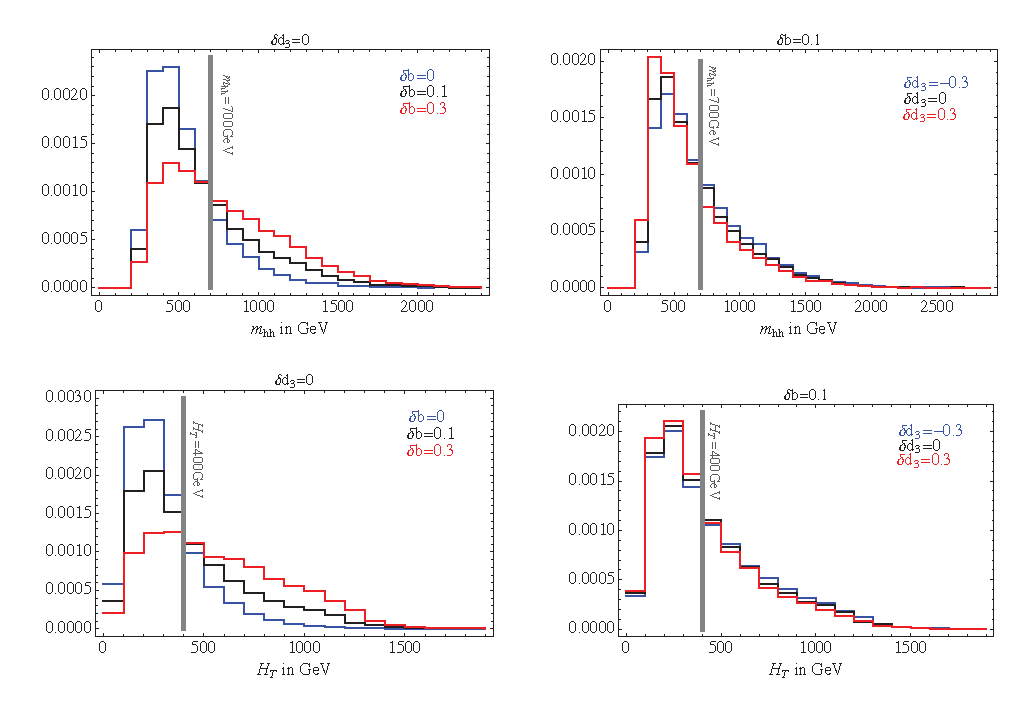
\includegraphics[width=1\textwidth]{theory/MhhHtDistribution}
\caption[]
{Normalized differential cross sections $d\sigma/dm_{hh}$ and $d\sigma/dH_{T}$ for \HepProcess{\Ppositron\Pelectron \to \Pneutrino\APneutrino hh} at the Compact Linear Collider, with \rootS{3} TeV after the identification cuts, for several values of $\delta_{b}$ and $\delta_{d_3}$. Plot is taken from \cite{Contino:2013gna}.}
\label{fig:theoryMhhHtDistribution}
\end{figure}

In the \Equation{eq:theoryGeneralHiggsCrossSection}, $a$, which is proportional to $g_{VVH}$, only entres as an overall factor. However, $a$ also appears in the definition of $\delta_{b}$ and $\delta_{d_3}$. To extract $\delta_{b}$ and $\delta_{d_3}$, $a$ should be a constant ideally. For a multi-TeV electron-positron collider, the cross section for single Higgs production is far greater than that of the double Higgs. \FIGURE{fig:theoryHiggsCrossSection} shows the comparison of the cross section as a function of the centre-of-mass energy. Therefore, $g_{VVH}$ and $a$ will be measured precisely before investigating the double Higgs production. For the purpose of measuring $g_{VVHH}$ and $g_{HHH}$ via double Higgs production, $a$ in the \Equation{eq:theoryGeneralHiggsCrossSection} can be treated as a constant.

\begin{figure}[!htbp]
\centering
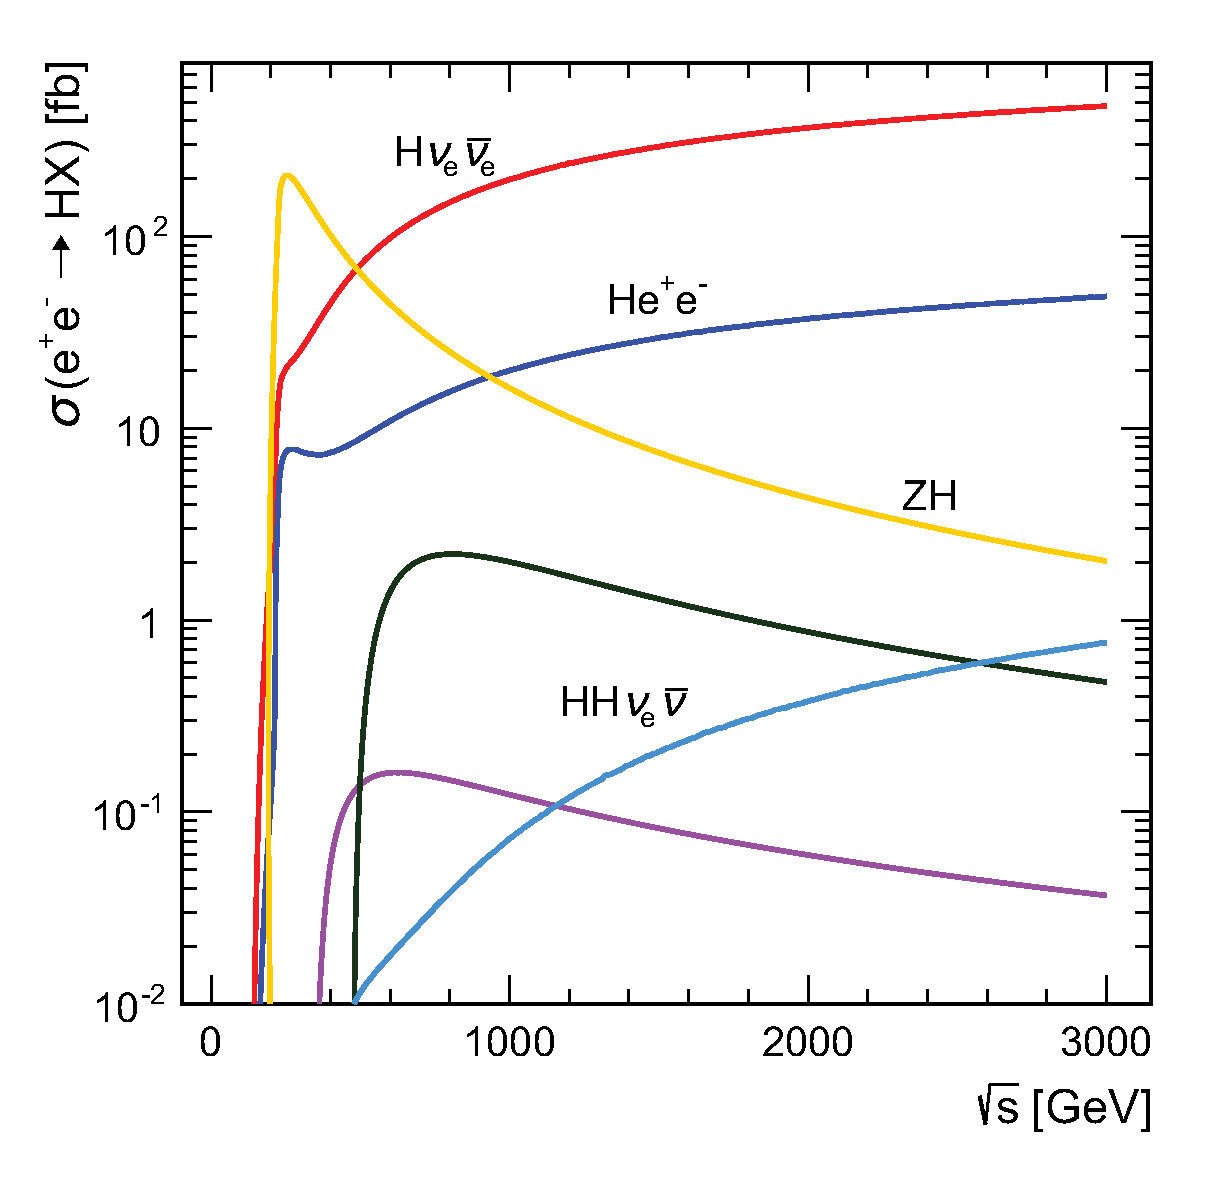
\includegraphics[width=0.45\textwidth]{theory/HiggsCLICcrossSection}
\caption[]
{Cross section as a function of centre-of-mass energy for the Higgs production processes at an electron-positron collider for a Higgs mass of 126GeV. The values shown correspond
to unpolarised beams and do not include the effect of beamstrahlung. Plot is taken from \cite{Abramowicz:2016zbo}.}
\label{fig:theoryHiggsCrossSection}
\end{figure}



%Photon - passage through matter. Photon electromagnetic shower

